\documentclass[12pt, titlepage]{article}
\usepackage{xcolor} % for different colour comments

%% Comments
\newif\ifcomments\commentstrue

\ifcomments
\newcommand{\authornote}[3]{\textcolor{#1}{[#3 ---#2]}}
\newcommand{\todo}[1]{\textcolor{red}{[TODO: #1]}}
\else
\newcommand{\authornote}[3]{}
\newcommand{\todo}[1]{}
\fi

\newcommand{\wss}[1]{\authornote{magenta}{SS}{#1}}
\newcommand{\ds}[1]{\authornote{blue}{DS}{#1}}

%% Graphics
\usepackage{float}
\usepackage{caption}
\usepackage{graphicx}
\usepackage{courier}
\graphicspath{ {images/} }

\begin{document}

\title{Smart Waiter User Guide} 
\author{Meraj Patel \#1137491 \\ Pavneet Jauhal \#1149311\\ Shan Perera \#1150394}
\date{\today}
\maketitle

\tableofcontents 

\listoffigures

\listoftables

\begin{table}[H]
\section*{Revision History}
\begin{tabular}{|c|c|}
\hline
\textbf{Date}  & \textbf{Comments} \\ \hline
February 26, 2016 &  First Draft. \\ 
\hline
February 27, 2016 & Create Account section complete. \\
\hline
February 28, 2016 & Account Setup complete \\
\hline
February 28, 2016 & Placing an Order complete \\
\hline
February 28, 2016 & Getting Started complete \\
\hline
\end{tabular}
\caption{Revision History Table}
\end{table}

\section{Introduction}
\subsection{What is Smart-Waiter?}
\subsection{Objectives of User Manual}

\section{Getting Started }
\subsection{System Requirements}
To use Smart-Waiter, your phone must be running Android's Ice Cream Sandwich (4.0.1) operating system or higher. Your device must also have at least 512MB of RAM. The minimum and recommended requirements for running Smart-Waiter are given below.
Minimum Requirements:
\begin{enumerate}
	\item Android OS Version: Ice Cream Sandwich (4.0.1)
	\item Resolution: 480 x 854 pixels (~195 PPI pixel density)
	\item Processor: 1.0 GHz
	\item Storage: 100MB
	\item RAM: 512MB
	\item Camera: 2.0 MP Front Facing Camera
	\item WLAN: WiFi 802.11 b/g/n OR HSPA compatible data service
\end{enumerate}

Recommended Requirements:
\begin{enumerate}
\item Android OS Version: Marshmallow (6.0)
	\item Resolution: 1440 x 2560 pixels (~575 PPI pixel density)
	\item Processor: Exynos 7420 Octacore (1.5 GHz Quad Core \& 2.1 GHz Quad Core)
	\item Storage: 100MB
	\item RAM: 3GB
	\item Camera: 16.0 MP Front Facing Camera
	\item WLAN: WiFi 802.11 b/g/n OR LTE compatible data service	
\end{enumerate}

\subsection{Installation Instructions}
Instructions for installing Smart-Waiter with 3 different methods are presented below. Currently, the only way to install Smart-Waiter is through Android Studio. Once the final revision is complete, installation using the application APK or through the Play Store will be available.

\textbf{\newline Installation through the Play Store:}
	\begin{enumerate}
		\item Open the Play Store application on your device.
		\item Press the Search Button
		\item Enter \emph{Smart Waiter} into the search field.
		\item Select \emph{Smart Waiter} from the search results.
		\item Press the \texttt{Install} button.		
	\end{enumerate}

\textbf{\newline Installation with APK:}
	\begin{enumerate}
		\item Download the APK file from the Smart-Waiter Git Repository
		\item Open your device's \emph{File Explorer} application
		\item Navigate to the folder where the APK file was saved
		\item Open the APK file using your device's \emph{File Explorer}
		\item Press the \texttt{Install} button
	\end{enumerate}

\textbf{\newline Installation with Android Studio:}
	\begin{enumerate}
		\item Checkout the Smart-Waiter Git Repository to a directory of 				your choice
		\item Open \emph{Android Studio}
		\item Select the \texttt{File} tab from the Menu
		\item Select \texttt{New Project >> Import Project...}
		\item Navigate to the folder where Smart-Waiter is saved
		\item Select the \texttt{build.gradle} file in the \emph{root} 					directory
		\item Wait for the project to build
		\item Plug your Android device in to your computer 
		\item Press the \texttt{Run 'app'} button or Press \texttt{Shift+F10}
		\item Select your Android device from the \emph{Choose a running device} section
		\begin{center}
			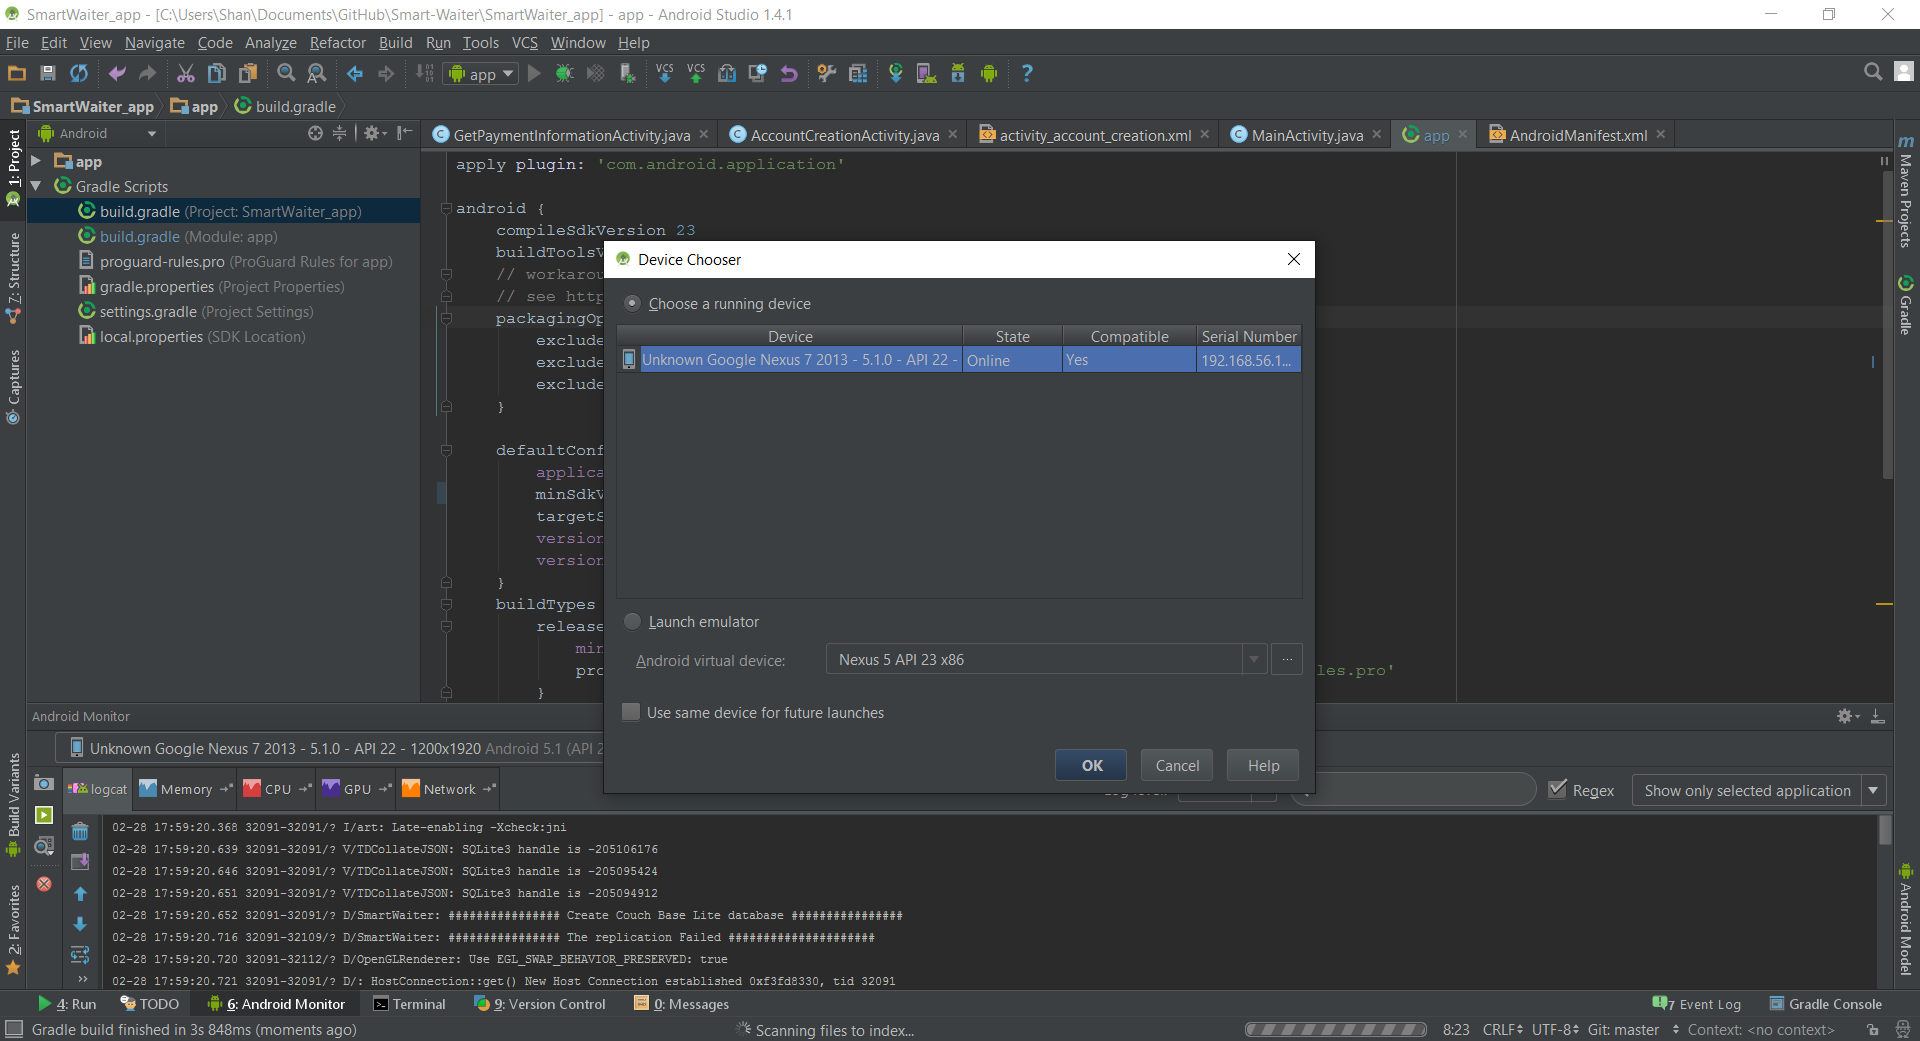
\includegraphics[width=1.0\textwidth]{android-studio.png}
		\end{center}
		\item Press the \texttt{OK} button		
	\end{enumerate}
You have successfully installed Smart-Waiter on your Android device.
\section{Account Setup}
\subsection{Creating an Account}
If this is the first time that Smart-Waiter is launched, you will be asked to create an account. You will be brought to the Account Creation screen as soon as Smart-Waiter is initialized. Your screen will look similar to Figure 1 below. 

\begin{center}
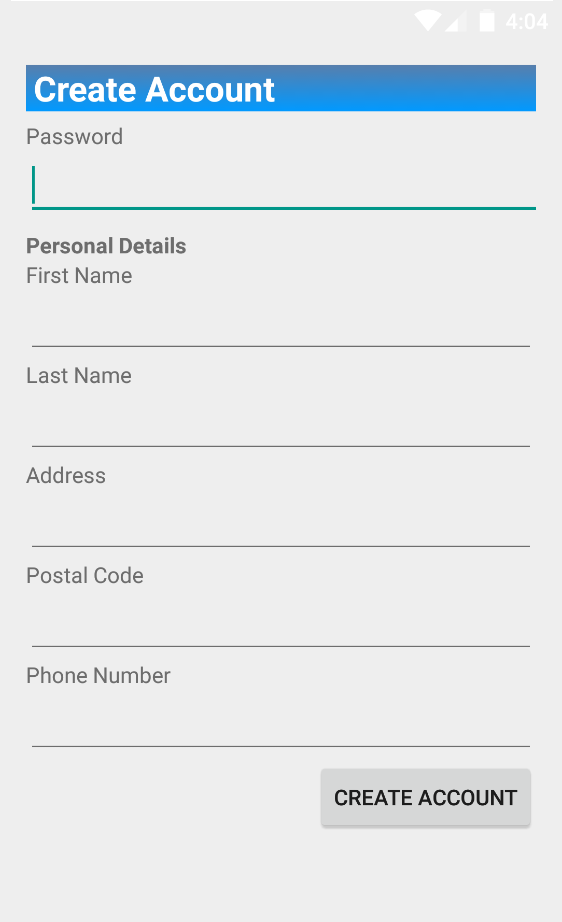
\includegraphics[width=0.5\textwidth]{accountCreation.png}
\linebreak Figure 1
\end{center}

The instructions to create an account are as follows: 
\begin{enumerate}
	\item Choose a password between 2-5 characters long.
	\item Enter your first name into the corresponding field.
	\item Enter your last name into the corresponding field.
	\item Enter the first line of your home address as it appears on your mail. Ex: \texttt{125 Royal Ave}
	\item Enter your postal code in the following format: \texttt{L4H 3Y4}
	\item Enter your phone number in the following format: \texttt{4165551911}
	\item Press the \texttt{Create Account} button.
\end{enumerate}

Your Smart-Waiter account has now been successfully created.
\subsection{Accessing Account Settings}
This feature is set to be implemented in our final revision. For the time being, a general walk-through is given using a generic android application settings module. To access your Account Settings in Smart-Waiter proceed with the following steps:

\begin{enumerate}
	\item Press the button with 3 horizontal white lines on the top right-			hand corner of the screen to bring up the Navigation menu, as seen 			in Figure 2: 
	
	\begin{center}
	
\includegraphics[width=0.05\textwidth]{ui-fragment-button.png}
	\linebreak Figure 2
	\end{center}

	\item Press the \texttt{Settings} button in the Navigation Menu as seen 	in Figure 3:

	\begin{center}
	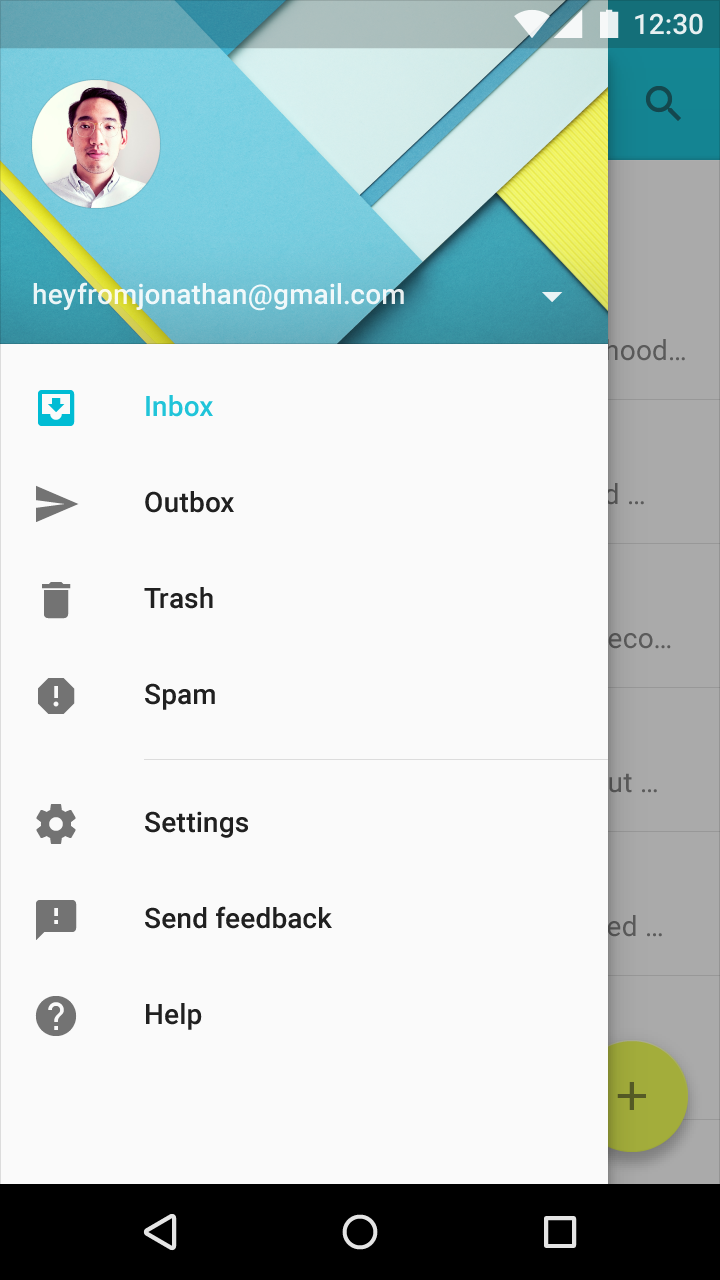
\includegraphics[width=0.4\textwidth]{nav-menu.png}
	\linebreak Figure 3
	\end{center}

\end{enumerate}

From here you can edit your Account Settings. You can perform the following actions in the settings page: \texttt{Change Password} and \texttt{Edit Personal Details}.

\textbf{Changing Your Password:}
	\begin{enumerate}
		\item Press the \texttt{Change Password} label.
		\item Enter your current password into the corresponding field
		\item Press the \texttt{Confirm} button
		\item Enter a new password between 2-5 characters
		\item Enter your new password again into the \texttt{Confirm Password} field
		\item Press the \texttt{Update Password} button.
	\end{enumerate}
	
\textbf{Editing Your Personal Details:}
	\begin{enumerate}
		\item Press the \texttt{Edit Personal Details} label.
		\item Enter your updated information into the corresponding field
		\begin{enumerate}
			\item \textbf{NOTE:} If you leave a field blank, the 						information for the corresponding field will not be updated.
		\end{enumerate}
		\item Press the \texttt{Save Changes} button.
	\end{enumerate}
\section{View Restaurant Menu}
\subsection{Scanning Barcode}
\subsection{Menu Layout}

\section{Placing an Order}
\subsection{Adding Item to Cart}
This section will walk-through how to add an item to your cart. In this case we are using the Chalet Bar and Grill Menu, however these instructions can be applied to any menu available through Smart-Waiter. Your screen will look similar to Figure 4 below. To learn how to add an item to your cart, proceed with the following instructions:
	\begin{enumerate}
		\item Press the label for the category of your choice. Ex: 						\texttt{Appetizers}

	\begin{center}
		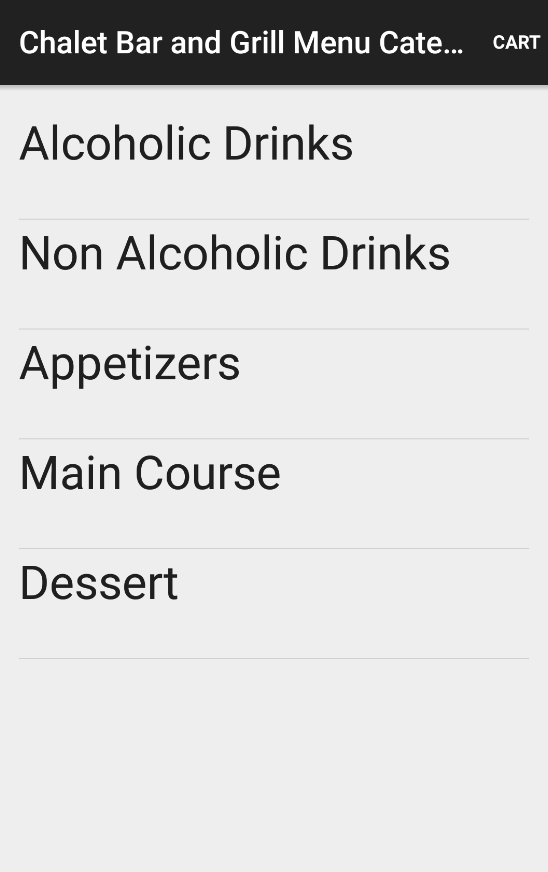
\includegraphics[width=0.5\textwidth]{main-menu.png}
		\linebreak Figure 4
	\end{center}

		\item Press the label for the menu item of your choice. Ex: 					\texttt{Autumn Spinach Salad}
		\begin{center}
			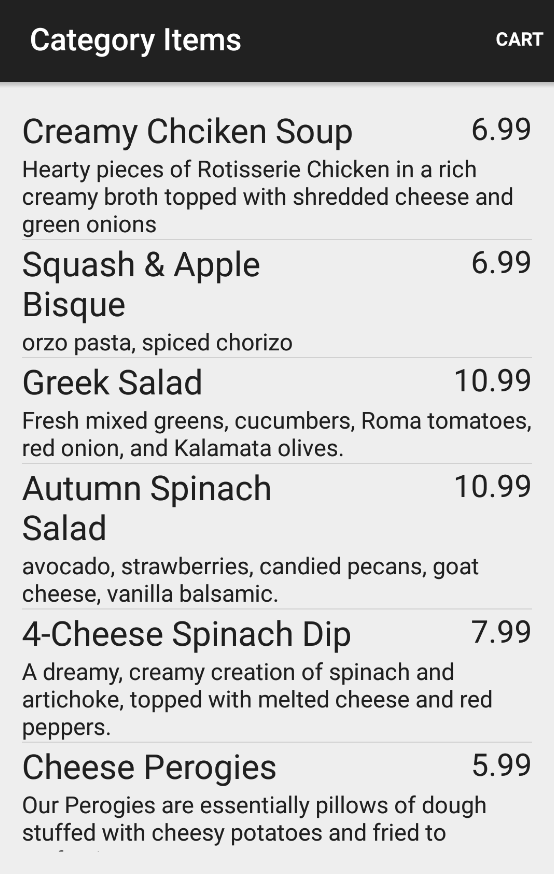
\includegraphics[width=0.5\textwidth]{appetizers.png}
			\linebreak Figure 5
		\end{center}				
		
		\item Enter any special instructions you may have for the menu 					item. Ex: \texttt{Easy on the salad dressing} - Refer to Figure 			6
		\begin{center}
			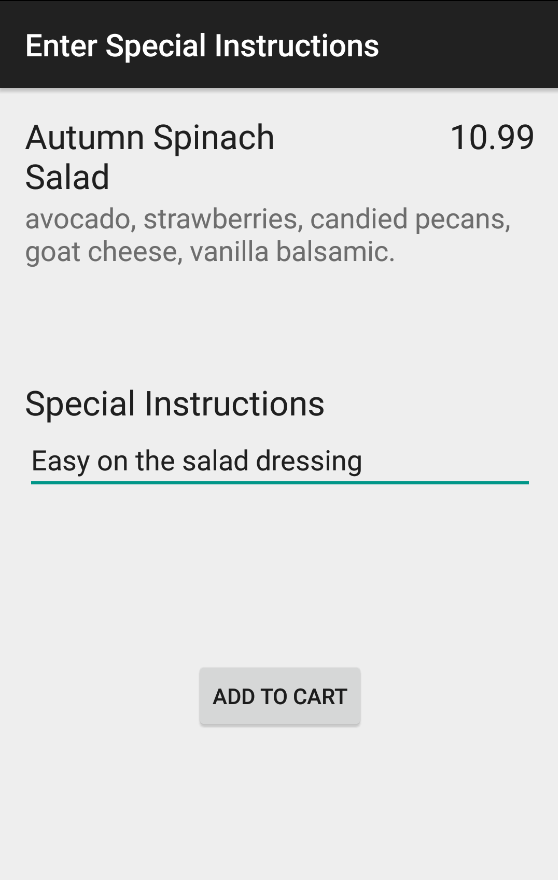
\includegraphics[width=0.5\textwidth]{special-instructions.png}
			\linebreak Figure 6
		\end{center}		
	
		\item Press the \texttt{Add To Cart} button
	\end{enumerate}

\subsection{Order Confirmation}
This section will guide you through the order confirmation process. We will continue with the Chalet Bar and Grill case we followed in the previous sections. These instructions can be applied to any menu available through Smart-Waiter. To learn how to confirm your order, proceed with the following instructions:

	\begin{enumerate}
		\item Press the \texttt{Cart} button on the top right corner of the 			application.
		\item Press the \texttt{Confirm Order} button
		\begin{center}
			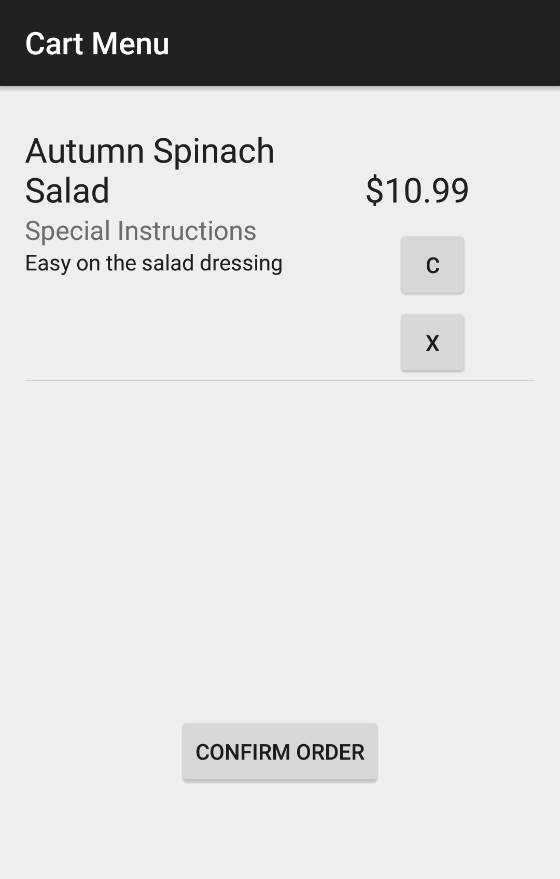
\includegraphics[width=0.5\textwidth]{confirm-order.png}
			\linebreak Figure 7
		\end{center}
		\item Press the \texttt{Proceed to Payment} button
	\end{enumerate}
	
	\textbf{Edit Special Instructions:}
	To edit the special instructions for a menu item, proceed to the Cart Menu by pressing the \texttt{Cart} button on the top right corner of the screen and follow these instructions:
	
	\begin{enumerate}
		\item Press the \texttt{C} button
		\item Update the \texttt{Special Instructions} field with your new instructions
		\item Press the \texttt{Modify Item} button
	\end{enumerate}
	
		\textbf{Remove Item from Cart:}
	To remove a menu item from your cart, proceed to the Cart Menu by pressing the \texttt{Cart} button on the top right corner of the screen and follow these instructions:
	
	\begin{enumerate}
		\item Press the \texttt{X} button
	\end{enumerate}

\subsection{Paying for an Order}
This section will guide you through the payment process. If you have not read the \emph{Order Confirmation} section yet, please do so now before moving forward with this guide. This tutorial assumes that you have added at least one menu item to your cart and have followed the main \emph{Order Confirmation} instructions up to step 3 where the user presses the \texttt{Proceed to Payment} button step. Your screen will look similar to Figure 8 below. To learn how to pay your order, proceed with the following instructions:

	\begin{center}
		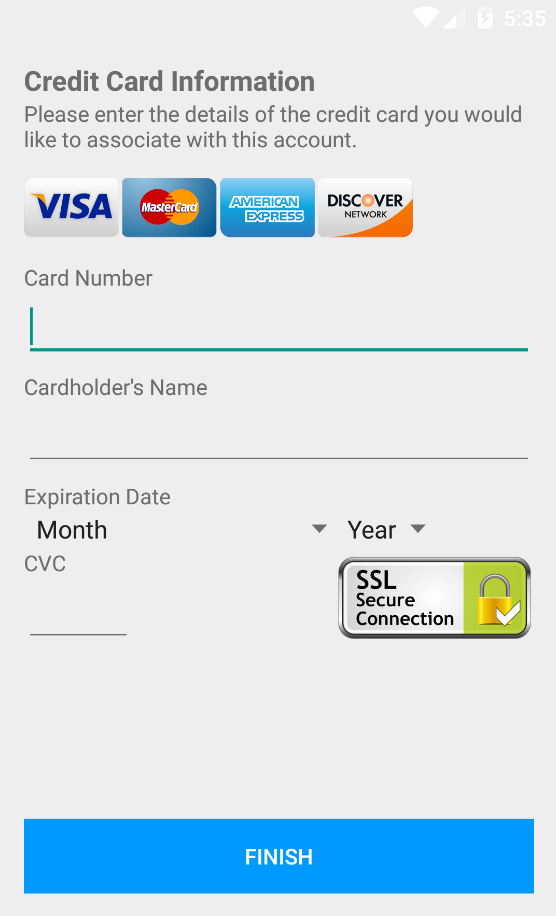
\includegraphics[width=0.5\textwidth]{cc.png}
		\linebreak Figure 8
	\end{center}
	\begin{enumerate}
		\item Enter your \emph{Credit Card Number} into the \texttt{Card 				Number}	field
		\item Enter the \emph{Cardholder's Name} into the corresponding 				field
		\item Enter the \emph{Expiration Date} using the dropdown list
		\item Enter the \emph{CVC} into the corresponding field
		\item Press the \texttt{Finish} button
	\end{enumerate}

\subsection{Submitting an Order}

\section{Troubleshooting}
\subsection{Overview}
\subsection{Barcode Scanning Error}
\subsection{Application Freeze}
\subsection{Frequently Asked Questions}



\end{document}